\section{Final testing and conclusions}\label{sec:conclusions}

Once we refined our model at the best could, we evaluated it against never seen data, by comparing the values predicted by the model, when the testing set is provided as input, against the true values of the annotations in the testing set. As already mentioned in section~\ref{sec:cross-validation}, once the final testing is done, we avoided going back to the model and make further tweaks, as this would have led to over-fitting.

For the final test we used the metrics of MSE and $R^2$-score (see section~\ref{sec:metrics}) and obtained the values reported in table~\ref{table:eval-metrics}. \todo{aggiungere considerazioni sui risultati}

\begin{table}[b]
	\centering
	\subcaptionbox{MSEs}{
		\begin{tabular}{lcccc}
			\toprule
			& valence mean & valence std & arousal mean & arousal std \\
			\midrule
			Ridge & 0.53 & 1.09 & 0.54 & 1.18 \\
			$\nu$-SVM & 0.58 & 1.00 & 0.49 & 1.09 \\
			K-neighbors & 0.62 & 1.00 & 0.61 & 1.08 \\
			\bottomrule
		\end{tabular}
	}
	\subcaptionbox{$R^2$-scores}{
		\begin{tabular}{lcccc}
			\toprule
			& valence mean & valence std & arousal mean & arousal std \\
			\midrule
			Ridge & 0.45 & -0.08 & 0.45 & -0.09 \\
			$\nu$-SVM & 0.40 & 0.01 & 0.50 & 0.00 \\
			K-neighbors & 0.35 & 0.01 & 0.39 & 0.00 \\
			\bottomrule
		\end{tabular}
	}
	\caption{Evaluation metrics}
	\label{table:eval-metrics}
\end{table}

We also extracted scatter plots comparing the predictions of each regressor against the true values of the testing set. In  figure~\ref{fig:eval-scatter} is depicted the case of \texttt{SVR}, which turned out to be the best model fitting the data.

\begin{figure}
	\centering
	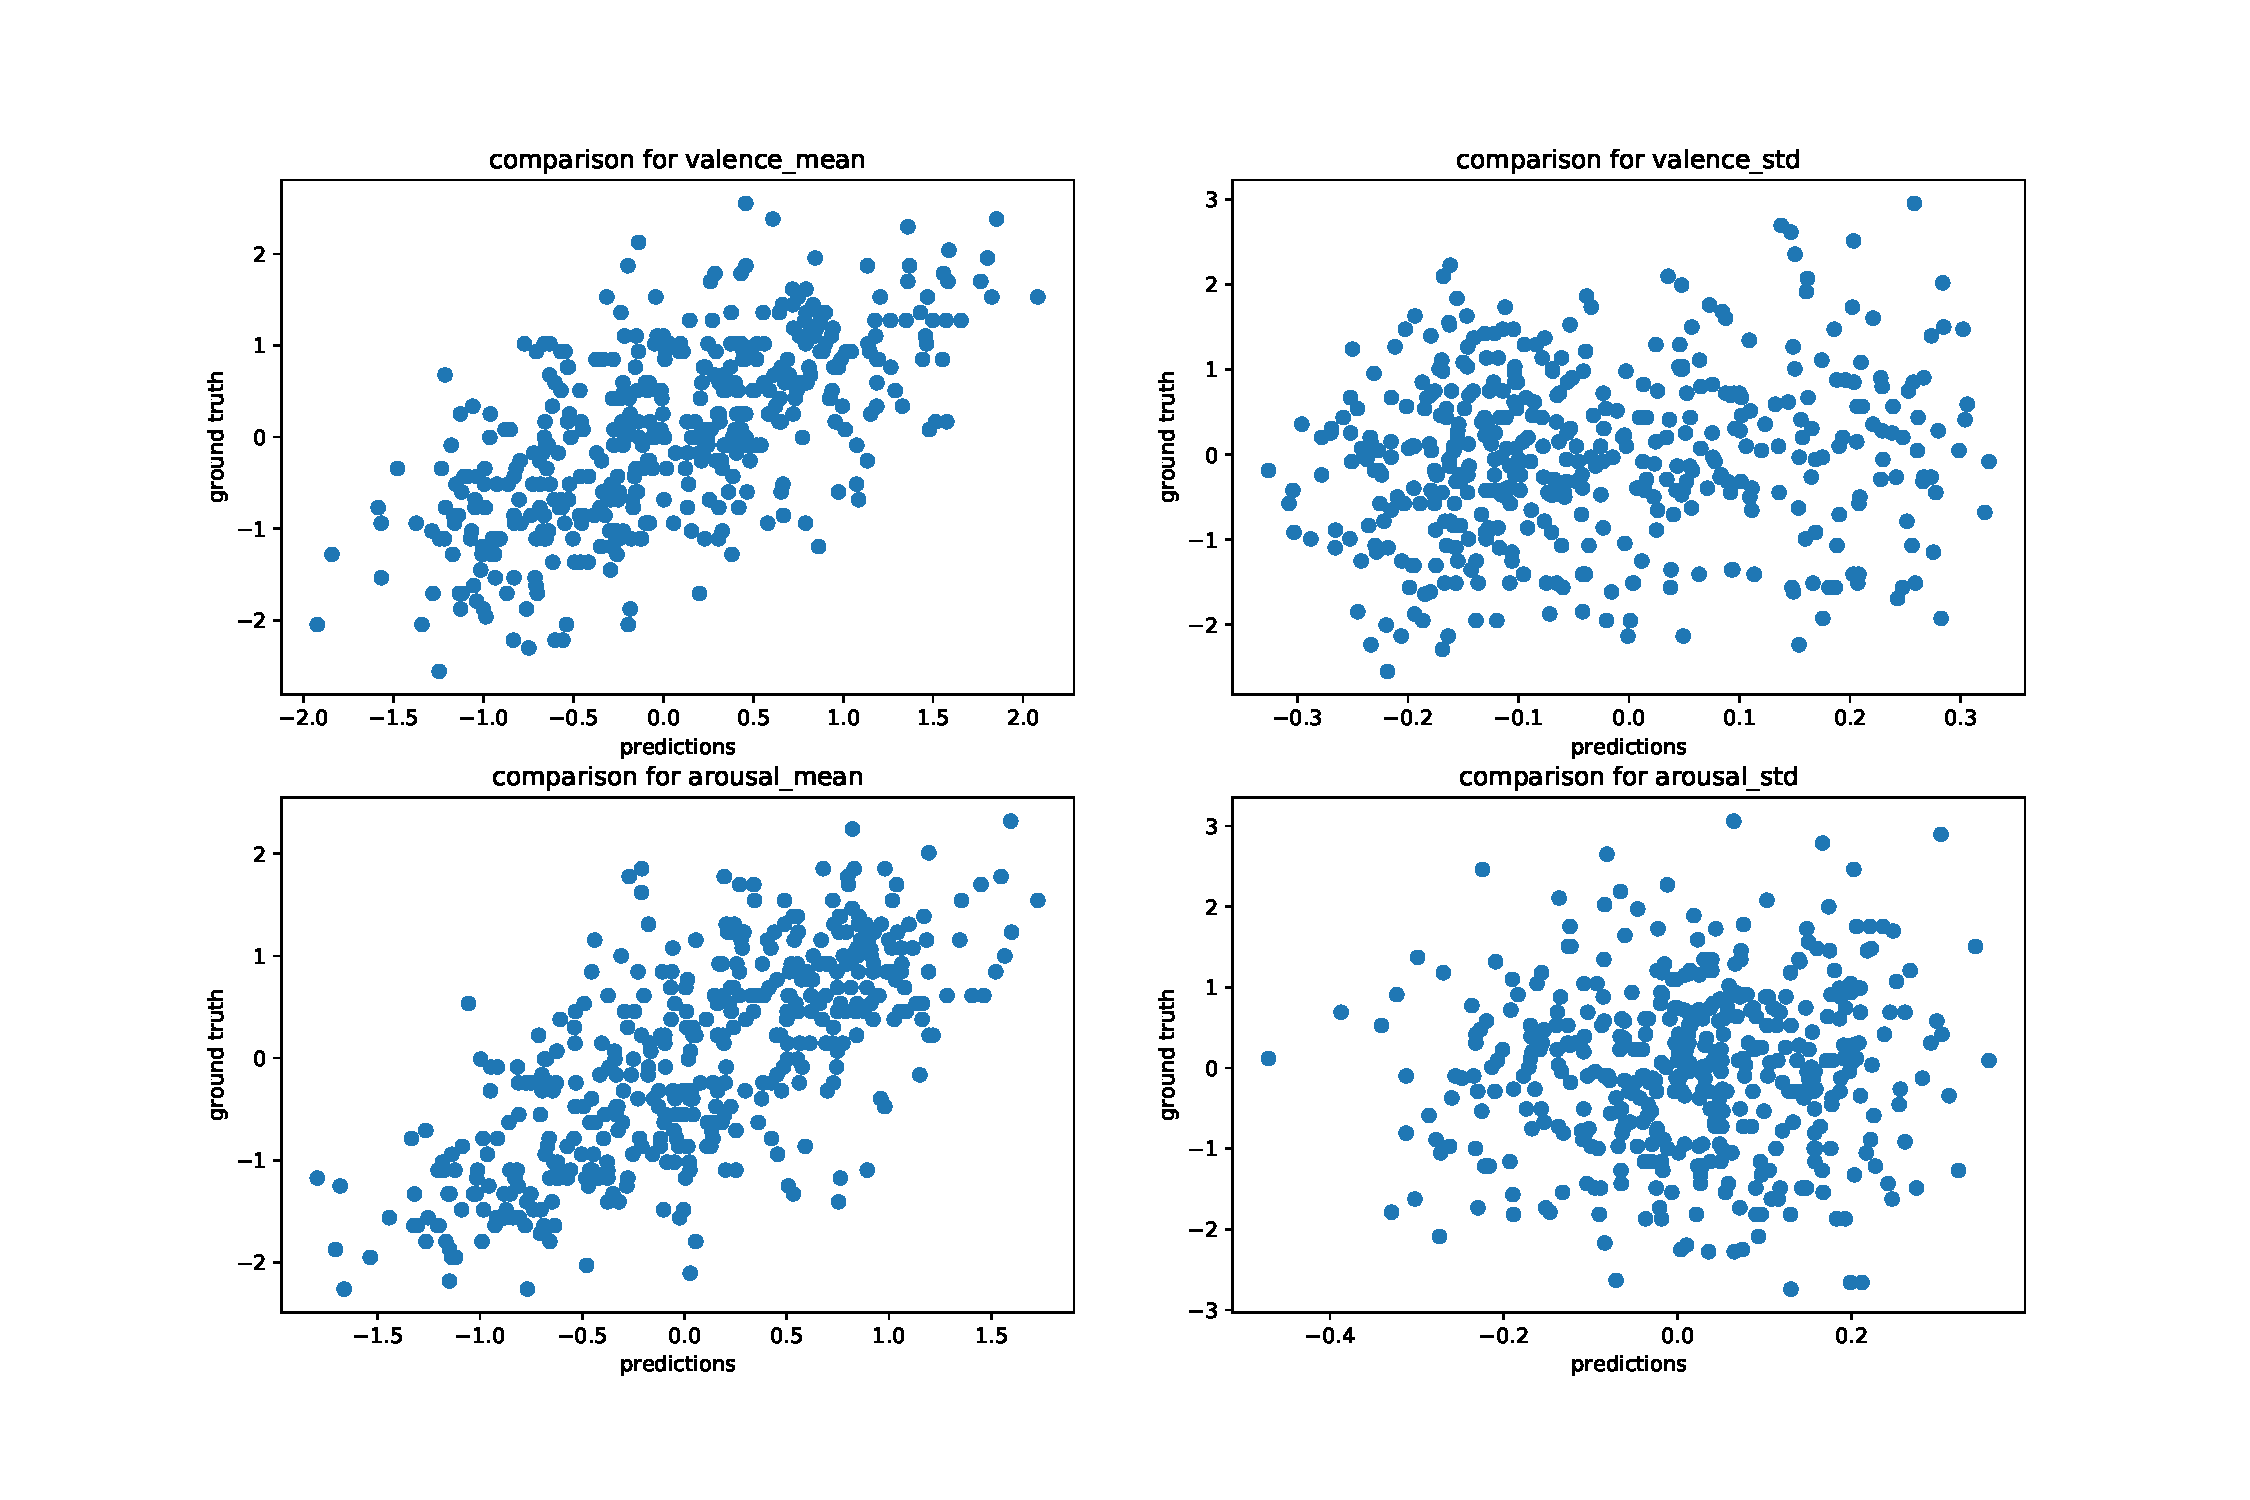
\includegraphics[width=\linewidth]{assets/predictions-scatter.pdf}
	\caption{predictions vs. ground-truth scatter for SVM regression}
	\label{fig:eval-scatter}
\end{figure}


\todo{da finire}